%\subsubsection{3D-Plots mit Durchschnittswerten gemittelt über die Tensorgröße}
%\begin{figure}[H]
%\centering
\begin{comment}
\begin{tikzpicture}
\begin{semilogyaxis}[height=0.40\textheight,width=0.40\textwidth,style={font=\footnotesize},grid=major,grid style={dotted},align=center,xlabel={Kontraktionsmodus},ylabel={Tensorstufe},title={TLib-LB-P3},scaled ticks=false,zticklabel=\pgfmathprintnumber{\tick},zlabel={Verhältnis},view={-45}{45}]
\addplot3[surf]
coordinates{(1.000,2.000,0.982) (1.000,3.000,0.997) (1.000,4.000,1.010) (1.000,5.000,0.994) (1.000,6.000,1.005) (1.000,7.000,1.016) (1.000,8.000,1.079) (1.000,9.000,1.020) (1.000,10.000,1.028) 

(2.000,2.000,1.154) (2.000,3.000,0.955) (2.000,4.000,1.100) (2.000,5.000,1.121) (2.000,6.000,1.120) (2.000,7.000,1.133) (2.000,8.000,1.113) (2.000,9.000,1.128) (2.000,10.000,1.130) 

(3.000,2.000,1.117) (3.000,3.000,1.117) (3.000,4.000,1.463) (3.000,5.000,1.703) (3.000,6.000,1.464) (3.000,7.000,1.087) (3.000,8.000,1.119) (3.000,9.000,1.169) (3.000,10.000,1.150) 

(4.000,2.000,1.080) (4.000,3.000,1.158) (4.000,4.000,1.048) (4.000,5.000,2.365) (4.000,6.000,2.296) (4.000,7.000,1.437) (4.000,8.000,1.071) (4.000,9.000,1.151) (4.000,10.000,1.168) 

(6.000,2.000,1.054) (6.000,3.000,1.067) (6.000,4.000,1.016) (6.000,5.000,1.010) (6.000,6.000,1.051) (6.000,7.000,3.183) (6.000,8.000,2.228) (6.000,9.000,1.477) (6.000,10.000,1.115) 

(7.000,2.000,1.044) (7.000,3.000,1.071) (7.000,4.000,1.038) (7.000,5.000,1.015) (7.000,6.000,1.006) (7.000,7.000,1.023) (7.000,8.000,3.158) (7.000,9.000,2.382) (7.000,10.000,1.495) 

(8.000,2.000,1.114) (8.000,3.000,1.079) (8.000,4.000,1.050) (8.000,5.000,1.009) (8.000,6.000,1.028) (8.000,7.000,1.013) (8.000,8.000,1.012) (8.000,9.000,3.395) (8.000,10.000,2.411) 

(9.000,2.000,1.120) (9.000,3.000,1.061) (9.000,4.000,1.057) (9.000,5.000,1.021) (9.000,6.000,1.014) (9.000,7.000,1.003) (9.000,8.000,1.010) (9.000,9.000,1.006) (9.000,10.000,3.396) 

(10.000,2.000,1.041) (10.000,3.000,1.096) (10.000,4.000,1.032) (10.000,5.000,1.005) (10.000,6.000,1.008) (10.000,7.000,1.009) (10.000,8.000,0.998) (10.000,9.000,1.004) (10.000,10.000,1.000) 

};\end{semilogyaxis}
\end{tikzpicture}
\begin{tikzpicture}
\begin{semilogyaxis}[height=0.40\textheight,width=0.40\textwidth,style={font=\footnotesize},grid=major,grid style={dotted},align=center,xlabel={Kontraktionsmodus},ylabel={Tensorstufe},title={TLib-LB-P3},scaled ticks=false,zticklabel=\pgfmathprintnumber{\tick},zlabel={Verhältnis},view={-45}{45}, zlabel={Standardfehler [\%]}]
\addplot3[surf]
coordinates{(1.000,2.000,5.451) (1.000,3.000,3.228) (1.000,4.000,8.175) (1.000,5.000,3.080) (1.000,6.000,3.225) (1.000,7.000,1.438) (1.000,8.000,30.441) (1.000,9.000,1.452) (1.000,10.000,1.074) 

(2.000,2.000,2.138) (2.000,3.000,16.525) (2.000,4.000,7.900) (2.000,5.000,2.428) (2.000,6.000,2.195) (2.000,7.000,1.702) (2.000,8.000,1.731) (2.000,9.000,0.897) (2.000,10.000,0.707) 

(3.000,2.000,2.063) (3.000,3.000,2.569) (3.000,4.000,10.874) (3.000,5.000,6.725) (3.000,6.000,4.033) (3.000,7.000,2.220) (3.000,8.000,1.740) (3.000,9.000,1.502) (3.000,10.000,1.183) 

(4.000,2.000,1.635) (4.000,3.000,2.539) (4.000,4.000,1.552) (4.000,5.000,9.760) (4.000,6.000,5.719) (4.000,7.000,4.239) (4.000,8.000,1.880) (4.000,9.000,1.341) (4.000,10.000,1.488) 

(6.000,2.000,3.395) (6.000,3.000,2.200) (6.000,4.000,1.342) (6.000,5.000,1.938) (6.000,6.000,11.238) (6.000,7.000,8.538) (6.000,8.000,7.640) (6.000,9.000,6.468) (6.000,10.000,2.271) 

(7.000,2.000,2.748) (7.000,3.000,1.064) (7.000,4.000,1.867) (7.000,5.000,1.438) (7.000,6.000,2.177) (7.000,7.000,3.816) (7.000,8.000,8.824) (7.000,9.000,7.080) (7.000,10.000,4.892) 

(8.000,2.000,3.384) (8.000,3.000,3.096) (8.000,4.000,1.983) (8.000,5.000,1.846) (8.000,6.000,1.515) (8.000,7.000,1.681) (8.000,8.000,1.318) (8.000,9.000,8.365) (8.000,10.000,6.922) 

(9.000,2.000,2.611) (9.000,3.000,2.846) (9.000,4.000,1.787) (9.000,5.000,1.367) (9.000,6.000,1.972) (9.000,7.000,1.925) (9.000,8.000,1.001) (9.000,9.000,1.373) (9.000,10.000,10.853) 

(10.000,2.000,4.929) (10.000,3.000,1.831) (10.000,4.000,5.071) (10.000,5.000,1.801) (10.000,6.000,1.721) (10.000,7.000,1.395) (10.000,8.000,1.134) (10.000,9.000,0.936) (10.000,10.000,1.147) 

};
\end{semilogyaxis}
\end{tikzpicture}
\end{comment}
%\caption{
%\footnotesize Dargestellt sind über die Tensorgröße gemittelten \textbf{Laufzeitverhältnisse} der \textbf{Tensor}"=\textbf{Vektor}"=\textbf{Multiplikation}. Verglichen wurde die Variante \textbf{TLib-SB-P3} mit den obigen Varianten.  Daten sind in \textbf{Floating-Point<Single>} codiert.
%\label{fig:ttv_surf_ratio_float}
%}
%\end{figure}
%\clearpage
%\begin{figure}[H]
%\centering
\begin{tikzpicture}
\begin{axis}[height=0.2\textheight,width=0.35\textwidth,style={font=\scriptsize},grid=major,grid style={dotted},align=center,xlabel={Mode},ylabel={Order},title={\ttt{TLIB-SB-PN:TCL}}, scaled ticks=false, xtick={2,4,6,8,10}, xticklabels={2,4,6,8,10}, ytick={2,4,6,8,10}, yticklabels={2,4,6,8,10}, point meta max=11, point meta min=0.3, zmin=0.3, zmax=11, ztick={0.3,6,11}, zticklabels={0.3,6,11}, zlabel={Speedup}, view={-35}{45}, xlabel style={yshift=2mm}, ylabel style={yshift=5mm}, zlabel style={yshift=-1mm,xshift=-4mm}, title style={yshift=-2mm}] % zlabel={Speedup},
\addplot3[surf] % , colormap = {whiteblack}{color(0cm)=(white);color(0.4cm) = (darkgray)}
coordinates{
(1.000,2.000,0.598) (1.000,3.000,0.353) (1.000,4.000,1.063) (1.000,5.000,1.080) (1.000,6.000,1.062) (1.000,7.000,1.063) (1.000,8.000,1.125) (1.000,9.000,1.143) (1.000,10.000,1.165) 

(2.000,2.000,2.293) (2.000,3.000,1.310) (2.000,4.000,5.824) (2.000,5.000,8.121) (2.000,6.000,9.064) (2.000,7.000,6.133) (2.000,8.000,4.079) (2.000,9.000,3.451) (2.000,10.000,2.660) 

(3.000,2.000,2.276) (3.000,3.000,2.807) (3.000,4.000,5.767) (3.000,5.000,8.622) (3.000,6.000,10.746) (3.000,7.000,9.111) (3.000,8.000,6.691) (3.000,9.000,4.403) (3.000,10.000,3.540) 

(4.000,2.000,2.215) (4.000,3.000,2.896) (4.000,4.000,9.064) (4.000,5.000,8.638) (4.000,6.000,10.956) (4.000,7.000,10.291) (4.000,8.000,8.933) (4.000,9.000,7.094) (4.000,10.000,4.333) 

(6.000,2.000,2.168) (6.000,3.000,2.874) (6.000,4.000,8.895) (6.000,5.000,9.485) (6.000,6.000,10.119) (6.000,7.000,10.372) (6.000,8.000,9.315) (6.000,9.000,8.763) (6.000,10.000,6.753) 

(7.000,2.000,2.142) (7.000,3.000,2.789) (7.000,4.000,8.987) (7.000,5.000,9.457) (7.000,6.000,9.973) (7.000,7.000,9.204) (7.000,8.000,8.927) (7.000,9.000,8.726) (7.000,10.000,6.796) 

(8.000,2.000,2.268) (8.000,3.000,2.840) (8.000,4.000,9.026) (8.000,5.000,9.388) (8.000,6.000,10.052) (8.000,7.000,9.112) (8.000,8.000,8.388) (8.000,9.000,8.623) (8.000,10.000,6.833) 

(9.000,2.000,2.273) (9.000,3.000,2.803) (9.000,4.000,9.270) (9.000,5.000,9.396) (9.000,6.000,9.973) (9.000,7.000,9.094) (9.000,8.000,8.328) (9.000,9.000,6.832) (9.000,10.000,6.598) 

(10.000,2.000,2.198) (10.000,3.000,2.906) (10.000,4.000,8.948) (10.000,5.000,9.283) (10.000,6.000,9.948) (10.000,7.000,9.104) (10.000,8.000,8.286) (10.000,9.000,6.870) (10.000,10.000,4.492) 

};
\end{axis}
\end{tikzpicture}
\begin{comment}
\begin{tikzpicture}
\begin{semilogyaxis}[height=0.40\textheight,width=0.40\textwidth,style={font=\footnotesize},grid=major,grid style={dotted},align=center,xlabel={Kontraktionsmodus},ylabel={Tensorstufe},title={TCL},scaled ticks=false,zticklabel=\pgfmathprintnumber{\tick},zlabel={Verhältnis},view={-45}{45}, zlabel={Standardfehler [\%]}]
\addplot3[surf]
coordinates{(1.000,2.000,243.785) (1.000,3.000,15.829) (1.000,4.000,7.786) (1.000,5.000,12.309) (1.000,6.000,9.437) (1.000,7.000,10.334) (1.000,8.000,13.714) (1.000,9.000,8.598) (1.000,10.000,12.101) 

(2.000,2.000,8.466) (2.000,3.000,17.903) (2.000,4.000,22.758) (2.000,5.000,22.889) (2.000,6.000,30.126) (2.000,7.000,31.795) (2.000,8.000,25.066) (2.000,9.000,27.036) (2.000,10.000,35.057) 

(3.000,2.000,8.407) (3.000,3.000,7.866) (3.000,4.000,14.591) (3.000,5.000,16.698) (3.000,6.000,20.918) (3.000,7.000,29.688) (3.000,8.000,37.285) (3.000,9.000,26.938) (3.000,10.000,24.724) 

(4.000,2.000,10.169) (4.000,3.000,8.511) (4.000,4.000,11.776) (4.000,5.000,15.344) (4.000,6.000,16.310) (4.000,7.000,21.971) (4.000,8.000,30.644) (4.000,9.000,40.653) (4.000,10.000,26.625) 

(6.000,2.000,5.559) (6.000,3.000,8.439) (6.000,4.000,11.357) (6.000,5.000,14.391) (6.000,6.000,18.876) (6.000,7.000,23.022) (6.000,8.000,29.309) (6.000,9.000,34.232) (6.000,10.000,44.289) 

(7.000,2.000,7.182) (7.000,3.000,8.485) (7.000,4.000,11.419) (7.000,5.000,14.765) (7.000,6.000,18.500) (7.000,7.000,26.051) (7.000,8.000,31.450) (7.000,9.000,33.456) (7.000,10.000,43.997) 

(8.000,2.000,8.429) (8.000,3.000,8.364) (8.000,4.000,11.085) (8.000,5.000,14.431) (8.000,6.000,18.301) (8.000,7.000,26.405) (8.000,8.000,35.182) (8.000,9.000,36.990) (8.000,10.000,45.332) 

(9.000,2.000,8.955) (9.000,3.000,8.311) (9.000,4.000,11.825) (9.000,5.000,14.624) (9.000,6.000,18.510) (9.000,7.000,25.709) (9.000,8.000,35.682) (9.000,9.000,43.135) (9.000,10.000,44.555) 

(10.000,2.000,9.298) (10.000,3.000,8.736) (10.000,4.000,11.393) (10.000,5.000,14.471) (10.000,6.000,18.138) (10.000,7.000,25.470) (10.000,8.000,35.090) (10.000,9.000,43.486) (10.000,10.000,43.972) 

};
\end{semilogyaxis}
\end{tikzpicture}
\end{comment}
\hfill
\begin{tikzpicture}
\begin{axis}[height=0.2\textheight,width=0.35\textwidth,style={font=\scriptsize},grid=major,grid style={dotted},align=center,xlabel={Mode},ylabel={Order},title={\ttt{TLIB-SB-PN:TBLIS}}, scaled ticks=false, xtick={2,4,6,8,10}, xticklabels={2,4,6,8,10}, ytick={2,4,6,8,10}, yticklabels={2,4,6,8,10}, point meta max=7, point meta min=1, zmin=1, zmax=7, ztick={1,4,7},zticklabels={1,4,7}, zlabel={Speedup}, view={-35}{45}, xlabel style={yshift=2mm}, ylabel style={yshift=5mm}, zlabel style={yshift=-1mm,xshift=-4mm}, title style={yshift=-2mm}] % zlabel={Speedup}, 
\addplot3[surf] %, colormap = {whiteblack}{color(0cm)=(white);color(0.4cm) = (darkgray)}
coordinates{
(1.000,2.000,3.929) (1.000,3.000,3.439) (1.000,4.000,3.270) (1.000,5.000,3.167) (1.000,6.000,3.348) (1.000,7.000,3.220) (1.000,8.000,3.195) (1.000,9.000,3.233) (1.000,10.000,3.401) 

(2.000,2.000,2.670) (2.000,3.000,1.134) (2.000,4.000,1.678) (2.000,5.000,2.607) (2.000,6.000,3.786) (2.000,7.000,3.727) (2.000,8.000,3.652) (2.000,9.000,3.771) (2.000,10.000,3.787) 

(3.000,2.000,2.582) (3.000,3.000,3.293) (3.000,4.000,1.876) (3.000,5.000,3.096) (3.000,6.000,4.284) (3.000,7.000,4.286) (3.000,8.000,4.272) (3.000,9.000,4.339) (3.000,10.000,4.385) 

(4.000,2.000,2.568) (4.000,3.000,3.345) (4.000,4.000,2.896) (4.000,5.000,3.144) (4.000,6.000,4.469) (4.000,7.000,4.572) (4.000,8.000,4.547) (4.000,9.000,5.130) (4.000,10.000,4.937) 

(6.000,2.000,2.486) (6.000,3.000,3.428) (6.000,4.000,3.230) (6.000,5.000,4.172) (6.000,6.000,4.794) (6.000,7.000,5.650) (6.000,8.000,5.314) (6.000,9.000,5.674) (6.000,10.000,5.829) 

(7.000,2.000,2.419) (7.000,3.000,3.332) (7.000,4.000,3.129) (7.000,5.000,4.419) (7.000,6.000,4.557) (7.000,7.000,4.888) (7.000,8.000,5.361) (7.000,9.000,6.215) (7.000,10.000,6.362) 

(8.000,2.000,2.563) (8.000,3.000,3.331) (8.000,4.000,3.277) (8.000,5.000,4.527) (8.000,6.000,4.599) (8.000,7.000,5.348) (8.000,8.000,5.240) (8.000,9.000,5.602) (8.000,10.000,6.221) 

(9.000,2.000,2.557) (9.000,3.000,3.178) (9.000,4.000,3.176) (9.000,5.000,4.326) (9.000,6.000,4.724) (9.000,7.000,4.824) (9.000,8.000,5.164) (9.000,9.000,5.142) (9.000,10.000,6.216) 

(10.000,2.000,2.576) (10.000,3.000,3.485) (10.000,4.000,3.359) (10.000,5.000,4.521) (10.000,6.000,4.802) (10.000,7.000,5.486) (10.000,8.000,5.086) (10.000,9.000,5.092) (10.000,10.000,5.120) 

};
\end{axis}
\end{tikzpicture}
\begin{comment}
\begin{tikzpicture}
\begin{semilogyaxis}[height=0.40\textheight,width=0.40\textwidth,style={font=\footnotesize},grid=major,grid style={dotted},align=center,xlabel={Kontraktionsmodus},ylabel={Tensorstufe},title={TBLIS},scaled ticks=false,zticklabel=\pgfmathprintnumber{\tick},zlabel={Verhältnis},view={-45}{45}, zlabel={Standardfehler [\%]}]
\addplot3[surf]
coordinates{
(1.000,2.000,30.875) (1.000,3.000,10.330) (1.000,4.000,14.420) (1.000,5.000,12.800) (1.000,6.000,10.042) (1.000,7.000,13.294) (1.000,8.000,13.407) (1.000,9.000,13.349) (1.000,10.000,14.095) 

(2.000,2.000,6.433) (2.000,3.000,9.374) (2.000,4.000,9.844) (2.000,5.000,7.192) (2.000,6.000,10.489) (2.000,7.000,9.820) (2.000,8.000,9.926) (2.000,9.000,8.278) (2.000,10.000,9.343) 

(3.000,2.000,5.952) (3.000,3.000,6.423) (3.000,4.000,8.412) (3.000,5.000,5.803) (3.000,6.000,9.627) (3.000,7.000,8.471) (3.000,8.000,8.588) (3.000,9.000,6.391) (3.000,10.000,6.309) 

(4.000,2.000,8.137) (4.000,3.000,7.703) (4.000,4.000,8.462) (4.000,5.000,7.036) (4.000,6.000,4.659) (4.000,7.000,9.085) (4.000,8.000,7.323) (4.000,9.000,14.395) (4.000,10.000,6.096) 

(6.000,2.000,6.367) (6.000,3.000,10.626) (6.000,4.000,8.311) (6.000,5.000,9.022) (6.000,6.000,11.997) (6.000,7.000,14.903) (6.000,8.000,6.575) (6.000,9.000,8.366) (6.000,10.000,9.731) 

(7.000,2.000,4.557) (7.000,3.000,7.531) (7.000,4.000,12.406) (7.000,5.000,14.416) (7.000,6.000,1.485) (7.000,7.000,11.412) (7.000,8.000,7.339) (7.000,9.000,17.697) (7.000,10.000,18.643) 

(8.000,2.000,5.336) (8.000,3.000,3.701) (8.000,4.000,10.332) (8.000,5.000,16.241) (8.000,6.000,1.249) (8.000,7.000,19.041) (8.000,8.000,13.738) (8.000,9.000,7.527) (8.000,10.000,19.412) 

(9.000,2.000,7.962) (9.000,3.000,2.953) (9.000,4.000,5.891) (9.000,5.000,12.281) (9.000,6.000,12.554) (9.000,7.000,5.072) (9.000,8.000,17.262) (9.000,9.000,12.306) (9.000,10.000,19.644) 

(10.000,2.000,10.958) (10.000,3.000,8.736) (10.000,4.000,12.500) (10.000,5.000,16.239) (10.000,6.000,10.174) (10.000,7.000,18.612) (10.000,8.000,14.279) (10.000,9.000,16.600) (10.000,10.000,11.908) 

};
\end{semilogyaxis}
\end{tikzpicture}
\end{comment}
%\caption{
%\footnotesize Dargestellt sind über die Tensorgröße gemittelten \textbf{Laufzeitverhältnisse} der \textbf{Tensor}"=\textbf{Vektor}"=\textbf{Multiplikation}. Verglichen wurde die Variante \textbf{TLib-SB-P3} mit den obigen Varianten.  Daten sind in \textbf{Floating-Point<Single>} codiert.
%\label{fig:ttv_surf_ratio_float}
%}
%\end{figure}
%\clearpage
%\begin{figure}[H]
%\centering
\hfill
\begin{tikzpicture}
\begin{axis}[height=0.2\textheight,width=0.33\textwidth,style={font=\scriptsize},grid=major,grid style={dotted},align=center,xlabel={Mode},ylabel={Order},title={\ttt{TLIB-SB-PN:EIGEN}}, scaled ticks=false, xtick={2,4,6,8,10}, xticklabels={2,4,6,8,10}, ytick={2,4,6,8,10}, yticklabels={2,4,6,8,10}, point meta max=20, point meta min=2, zmin=2, zmax=20, ztick={2,11,20},zticklabels={2,11,20}, zlabel={Speedup}, view={-35}{45}, xlabel style={yshift=2mm}, ylabel style={yshift=5mm}, zlabel style={yshift=-1mm,xshift=-4mm}, title style={yshift=-2mm}] % 
\addplot3[surf] %, colormap = {whiteblack}{color(0cm)=(white);color(0.4cm) = (darkgray)}
coordinates{
%(1.000,2.000,50.917) (1.000,3.000,155.501) (1.000,4.000,282.556) (1.000,5.000,356.463) (1.000,6.000,433.352) (1.000,7.000,494.885) (1.000,8.000,568.860) (1.000,9.000,668.150) (1.000,10.000,751.009) 

(2.000,2.000,2.445) (2.000,3.000,1.700) (2.000,4.000,3.392) (2.000,5.000,6.069) (2.000,6.000,9.580) (2.000,7.000,10.676) (2.000,8.000,11.612) (2.000,9.000,13.405) (2.000,10.000,14.937) 

(3.000,2.000,2.408) (3.000,3.000,3.162) (3.000,4.000,3.109) (3.000,5.000,5.893) (3.000,6.000,9.218) (3.000,7.000,10.406) (3.000,8.000,11.515) (3.000,9.000,13.280) (3.000,10.000,14.915) 

(4.000,2.000,2.348) (4.000,3.000,3.145) (4.000,4.000,3.763) (4.000,5.000,5.741) (4.000,6.000,9.051) (4.000,7.000,10.329) (4.000,8.000,11.565) (4.000,9.000,13.258) (4.000,10.000,14.852) 

(6.000,2.000,2.318) (6.000,3.000,3.152) (6.000,4.000,3.661) (6.000,5.000,6.989) (6.000,6.000,9.878) (6.000,7.000,10.346) (6.000,8.000,11.264) (6.000,9.000,12.965) (6.000,10.000,14.628) 

(7.000,2.000,2.262) (7.000,3.000,3.098) (7.000,4.000,3.740) (7.000,5.000,7.057) (7.000,6.000,9.762) (7.000,7.000,12.714) (7.000,8.000,11.102) (7.000,9.000,13.100) (7.000,10.000,14.657) 

(8.000,2.000,2.380) (8.000,3.000,3.141) (8.000,4.000,3.746) (8.000,5.000,7.065) (8.000,6.000,9.885) (8.000,7.000,12.507) (8.000,8.000,14.936) (8.000,9.000,13.111) (8.000,10.000,14.575) 

(9.000,2.000,2.402) (9.000,3.000,3.093) (9.000,4.000,3.803) (9.000,5.000,7.012) (9.000,6.000,9.727) (9.000,7.000,12.643) (9.000,8.000,14.936) (9.000,9.000,17.080) (9.000,10.000,14.586) 

(10.000,2.000,2.283) (10.000,3.000,3.247) (10.000,4.000,3.756) (10.000,5.000,6.923) (10.000,6.000,9.708) (10.000,7.000,12.597) (10.000,8.000,15.039) (10.000,9.000,17.122) (10.000,10.000,18.729) 

};
\end{axis}
\end{tikzpicture}
\begin{comment}
\begin{tikzpicture}
\begin{semilogyaxis}[height=0.40\textheight,width=0.40\textwidth,style={font=\footnotesize},grid=major,grid style={dotted},align=center,xlabel={Kontraktionsmodus},ylabel={Tensorstufe},title={EIGEN},scaled ticks=false,zticklabel=\pgfmathprintnumber{\tick},zlabel={Verhältnis},view={-45}{45}, zlabel={Standardfehler [\%]}]
\addplot3[surf]
coordinates{(1.000,2.000,15.514) (1.000,3.000,6.702) (1.000,4.000,4.754) (1.000,5.000,6.353) (1.000,6.000,11.672) (1.000,7.000,12.338) (1.000,8.000,10.605) (1.000,9.000,7.517) (1.000,10.000,2.536) 

(2.000,2.000,1.697) (2.000,3.000,11.794) (2.000,4.000,9.822) (2.000,5.000,2.911) (2.000,6.000,1.333) (2.000,7.000,1.947) (2.000,8.000,1.959) (2.000,9.000,1.941) (2.000,10.000,1.633) 

(3.000,2.000,1.838) (3.000,3.000,1.506) (3.000,4.000,5.541) (3.000,5.000,3.561) (3.000,6.000,2.464) (3.000,7.000,2.012) (3.000,8.000,1.034) (3.000,9.000,1.117) (3.000,10.000,2.227) 

(4.000,2.000,3.486) (4.000,3.000,1.818) (4.000,4.000,1.157) (4.000,5.000,2.392) (4.000,6.000,1.784) (4.000,7.000,1.690) (4.000,8.000,1.336) (4.000,9.000,0.834) (4.000,10.000,1.551) 

(6.000,2.000,2.935) (6.000,3.000,1.827) (6.000,4.000,2.172) (6.000,5.000,2.022) (6.000,6.000,1.205) (6.000,7.000,1.714) (6.000,8.000,1.225) (6.000,9.000,0.659) (6.000,10.000,1.399) 

(7.000,2.000,1.789) (7.000,3.000,1.862) (7.000,4.000,1.279) (7.000,5.000,1.587) (7.000,6.000,2.280) (7.000,7.000,1.392) (7.000,8.000,0.969) (7.000,9.000,0.997) (7.000,10.000,2.441) 

(8.000,2.000,3.046) (8.000,3.000,2.416) (8.000,4.000,0.794) (8.000,5.000,2.263) (8.000,6.000,1.698) (8.000,7.000,1.646) (8.000,8.000,1.493) (8.000,9.000,0.638) (8.000,10.000,1.570) 

(9.000,2.000,3.033) (9.000,3.000,2.356) (9.000,4.000,1.047) (9.000,5.000,2.129) (9.000,6.000,1.745) (9.000,7.000,1.793) (9.000,8.000,1.726) (9.000,9.000,1.625) (9.000,10.000,1.024) 

(10.000,2.000,3.192) (10.000,3.000,1.636) (10.000,4.000,2.416) (10.000,5.000,2.726) (10.000,6.000,1.694) (10.000,7.000,1.618) (10.000,8.000,1.426) (10.000,9.000,1.348) (10.000,10.000,9.321) 

};
\end{semilogyaxis}
\end{tikzpicture}
\end{comment}
%\caption{
%\footnotesize Dargestellt sind über die Tensorgröße gemittelten \textbf{Laufzeitverhältnisse} der \textbf{Tensor}"=\textbf{Vektor}"=\textbf{Multiplikation}. Verglichen wurde die Variante \textbf{TLib-SB-P3} mit den obigen Varianten.  Daten sind in \textbf{Floating-Point<Single>} codiert.
%\label{fig:ttv_surf_ratio_float}
%}
%\end{figure}
